% superlight clients
% sidechains
\section{Our Contributions}
\subsection{Superblocks}


\begin{figure}
    \caption{The probabilistic hierarchical blockchain.
    Higher levels have achieved a higher difficulty during
    mining. All blocks are connected to the genesis block $G$.}
    \centering
    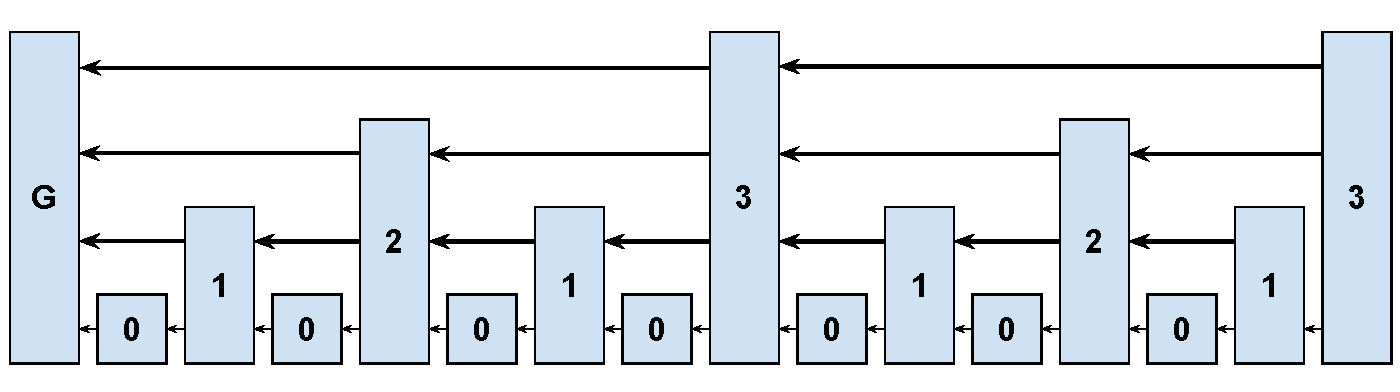
\includegraphics[width=0.7\columnwidth,keepaspectratio]{chapters/introduction/figures/hierarchical-ledger-span.pdf}
    \label{fig.hierarchy}
\end{figure}

The algorithm for this construction is shown in
Algorithm~\ref{alg.interlink-set}~\cite{compactsuperblocks}. The
interlink set of the Genesis block is, by definition, empty. The algorithm
describes how the interlink can be updated once a block is found. The new
interlink is then included in the next block. This construction ensures that
every block contains a direct pointer to its most recent $\mu$-superblock
ancestor, for every $\mu \in \mathbb{N}$.

\import{./}{chapters/superlight/algorithms/alg.interlink-set-update.tex}

The \textsf{updateInterlinkSet} algorithm accepts a block $B'$, which already has an
interlink data structure defined on it. The function evaluates the
interlink data structure which needs to be included as part of the next block.
It copies the existing interlink data structure from level $\textsf{level}(B')$
and adds the reference $H(B')$.
\todo{continuity}

\todo{NIPoPoWs}
\todo{applications to superlight wallets}
\todo{applications to sidechains}
\todo{applications to logspace mining}
\todo{the variable difficulty and $\Delta$-delay setting}
\todo{proofs of stake}
\todo{application: superlight clients}
\todo{application: sidechains}
\todo{application: logspace mining}

\subsection{Summary of Contributions}
A summary of our contributions and their dependencies, with annotations
indicating where they are presented in this thesis, is visually illustrated in
Figure~\ref{fig.contributions}.

In summary, in this thesis we solve the problem of \emph{consensus compression}
for all decentralized blockchain consensus mechanisms. \textbf{For
proof-of-work}, we introduce the NIPoPoWs primitive (Chapter 3) and we give two
superblock-based constructions of succinct NIPoPoWs protocols in the Backbone
model: First the \emph{charity} construction (Chapter~\ref{chapter:work}), and
second the \emph{distill} construction (Chapter~\ref{chapter:variable}
and~\ref{chapter:superlight}). In the static synchronous model
(Chapter~\ref{chapter:work}), we prove our charity construction with
\emph{goodness} secure against $\frac{1}{2}$ adversaries, but succinct only in
the optimistic setting. Our charity construction \emph{without goodness} as well
as our distill construction are both secure and succinct against $\frac{1}{3}$
adversaries (Chapter~\ref{chapter:variable}). In the synchronous variable model
(Chapter~\ref{chapter:variable}), our distill construction is secure against a
$\frac{1}{3}$ adversary as long as difficulty is non-decreasing. Our charity
without goodness construction is secure against a $\frac{1}{3}$ adversary even
if difficult is not limited to non-decreasing. Both are succinct as long as
difficulty is not exponentially decreasing. Lastly, in the $\Delta$-bounded
delay setting (Chapter~\ref{chapter:variable}), both constructions are secure
and succinct under the same limitations, but only against a $\frac{1}{4}$
adversary. We give concrete parameter recommendations and run experiments and
simulations indicatively for the charity construction of
Chapter~\ref{chapter:work}. \textbf{For proof-of-stake}, we construct the ATMs
primitive and give signature-based construction (Chapter~\ref{chapter:stake}).
These are secure in the Ouroboros model, but offer only constant improvements
over full clients and hence do not achieve asymptotic succinctness.

We make use of these primitives to build \textbf{cross-chain transfer}
applications, which give rise to interoperability among blockchains, allowing
generic information transfer among work/work, work/stake, and stake/stake
chains. We give the definition of what constitutes a secure sidechain protocol
(Chapter~\ref{chapter:sidechains}) and put forth cross-chain protocols which we
prove secure. Our protocols can work natively or by leveraging smart contract
functionality. We show how they can be utilized to create one-way and two-way
pegs and discuss several deployment mechanisms which allow them to be deployed
as soft forks or better. Our protocols can also be used to build superlight
clients. Lastly, we show that our proof-of-work protocols specifically can be
utilized to build logarithmic-space miners (Chapter~\ref{chapter:superlight}),
providing exponential improvements over the state and communication complexity
of existing blockchain protocols.

\begin{figure}
    \caption{
      A roadmap of this thesis' structure.
      Our underlying model is shown above the double line.
      Our contributions are shown below the double line and comprise consensus
      compression primitives (above the dashed line) and their applications
      (below the dashed line). The respective chapters are indicated next to
      each topic.
    }
    \centering
    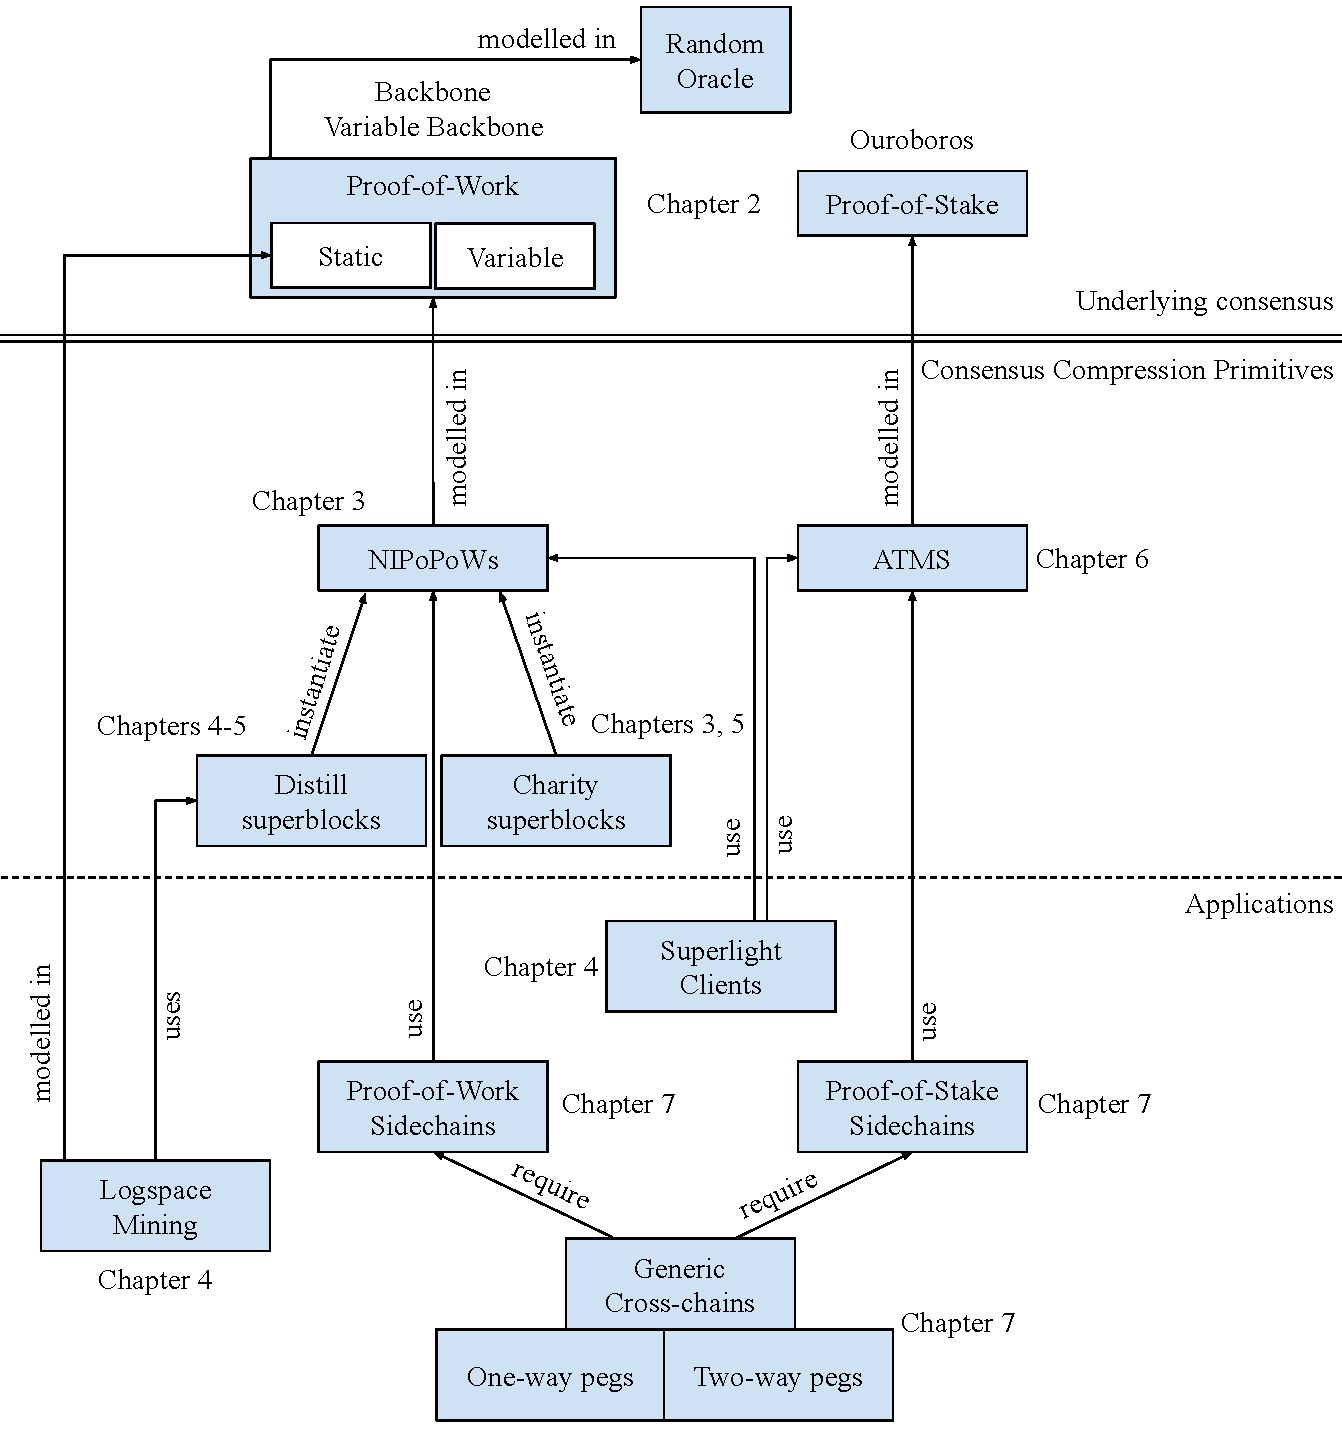
\includegraphics[width=\columnwidth,keepaspectratio]{chapters/introduction/figures/contributions.pdf}
    \label{fig.contributions}
\end{figure}
